\documentclass{ansarticle-preprint}
%\usepackage{ucs}
\usepackage[utf8]{inputenc}
\usepackage{amsmath}
%\usepackage{cite}
\usepackage{anslistings}
\usepackage{multicol}
\usepackage{pdfsync}

\usepackage{pgfplots}
\usepackage{pgfplotstable}

\usepackage{fontenc}
\usepackage{graphicx}
\usepackage{xspace}

\usepackage{siunitx}

\usepackage{floatflt}

\usepackage{multirow}

%\renewcommand{\baselinestretch}{2.0}

\usepackage[normalem]{ulem}

\usepackage{todonotes}

\pgfplotsset{compat=1.9}
\definecolor{gnuplot@lightblue}{RGB}{87,181,232}
\definecolor{gnuplot@green}{RGB}{0,158,115}
\definecolor{gnuplot@purple}{RGB}{148,0,212}

\newcommand{\specialword}[1]{\texttt{#1}}
\newcommand{\dealii}{{\specialword{deal.II}}\xspace}
\newcommand{\pfrst}{{\specialword{p4est}}\xspace}
\newcommand{\trilinos}{{\specialword{Trilinos}}\xspace}
\newcommand{\aspect}{\specialword{Aspect}\xspace}
\newcommand{\petsc}{\specialword{PETSc}\xspace}
\newcommand{\cmake}{{\specialword{CMake}}\xspace}
\newcommand{\candi}{{\specialword{candi}}\xspace}



\usetikzlibrary{shapes.misc}
\tikzset{cross/.style={cross out, draw=black, minimum size=2*(#1-\pgflinewidth), inner sep=0pt, outer sep=0pt},
%default radius will be 1pt.
cross/.default={2pt}}

%
% Author list -- please add yourself in both places below (in
%                alphabetical order) if you think that your
%                contributions to the last release warrant this
%

\hypersetup{
  pdfauthor={
    Daniel Arndt,
    Wolfgang Bangerth,
    Bruno Blais,
    Marc Fehling,
    Rene Gassm{\"o}ller
    Timo Heister,
    Luca Heltai,
    Uwe K{\"o}cher,
    Martin Kronbichler,
    Matthias Maier,
    Peter Munch,
    Jean-Paul Pelteret,
    Sebastian Proell,
    Konrad Simon,
    Bruno Turcksin,
    David Wells,
    Jiaqi Zhang
  },
  pdftitle={The deal.II Library, Version 9.3, 2021},
}

\title{The \dealii{} Library, Version 9.3}

 \author[1*]{Daniel Arndt}
 \affil[1]{Scalable Algorithms and Coupled Physics Group,
   Computational Sciences and Engineering Division,
   Oak Ridge National Laboratory, 1 Bethel Valley Rd.,
   TN 37831, USA.
   \texttt{arndtd/turcksinbr@ornl.gov}}

 \author[2,3]{Wolfgang~Bangerth}
 \affil[2]{Department of Mathematics, Colorado State University, Fort
   Collins, CO 80523-1874, USA.
   \texttt{bangerth/marc.fehling@colostate.edu}}
 \affil[3]{Department of Geosciences, Colorado State University, Fort
   Collins, CO 80523, USA.}

\author[4]{Bruno Blais}
\affil[4]{Research Unit for Industrial Flows Processes (URPEI), Department of Chemical Engineering,
          Polytechnique Montréal,
          PO Box 6079, Stn Centre-Ville, Montréal, Québec, Canada, H3C 3A7.
          {\texttt{bruno.blais@polymtl.ca}}}


\author[2]{Marc~Fehling}

\author[5]{Rene~Gassm{\"o}ller}
\affil[5]{Department of Geological Sciences,
   University of Florida,
   1843 Stadium Road,
   Gainesville, FL, 32611, USA.
  {\texttt{rene.gassmoeller@ufl.edu}}}

\author[6]{Timo~Heister}
 \affil[6]{School of Mathematical and Statistical Sciences,
   Clemson University,
   Clemson, SC, 29634, USA
   {\texttt{heister/jiaqi2@clemson.edu}}}

\author[7]{Luca~Heltai}
\affil[7]{SISSA,
   International School for Advanced Studies,
   Via Bonomea 265,
   34136, Trieste, Italy.
   {\texttt{luca.heltai@sissa.it}}}

\author[8]{Uwe~K{\"o}cher}
\affil[8]{Chair of Numerical Mathematics,
  Helmut-Schmidt-University,
  University of the Federal Armed Forces Hamburg,
  Holstenhofweg~85, 22043 Hamburg, Germany.
  {\texttt{uwe.koecher@hsu-hh.de}}}

 \author[9,10]{Martin~Kronbichler}
 \affil[9]{Institute for Computational Mechanics,
   Technical University of Munich,
   Boltzmannstr.~15, 85748 Garching, Germany.
   {\texttt{kronbichler/munch/proell@lnm.mw.tum.de}}}
 \affil[10]{Department of Information Technology,
   Uppsala University,
   Box 337, 751\,05 Uppsala, Sweden.
   {\texttt{martin.kronbichler@it.uu.se}}}

\author[11]{Matthias~Maier}
\affil[11]{Department of Mathematics,
  Texas A\&M University,
  3368 TAMU,
  College Station, TX 77845, USA.
  {\texttt{maier@math.tamu.edu}}}

\author[9,12]{Peter Munch}
 \affil[12]{Institute of Material Systems Modeling,
 Helmholtz-Zentrum Hereon,
 Max-Planck-Str. 1, 21502 Geesthacht, Germany.
   {\texttt{peter.muench@hereon.de}}}


\author[13]{Jean-Paul~Pelteret}
\affil[13]{Independent researcher.
{\texttt{jppelteret@gmail.com}}}

\author[9]{Sebastian~Proell}

\author[14]{Konrad Simon}
  \affil[14]{Department of Mathematics/Center
  for Earth System Research and Sustainability (CEN), University of
  Hamburg, Grindelberg 5, 20144 Hamburg, Germany.
  \texttt{konrad.simon@uni-hamburg.de}}

\author[1*]{Bruno~Turcksin}

\author[15]{David Wells}
\affil[15]{Department of Mathematics, University of North Carolina,
  Chapel Hill, NC 27516, USA.
  {\texttt{drwells@email.unc.edu}}}
  
\author[6]{Jiaqi~Zhang}

\renewcommand{\labelitemi}{--}


\begin{document}
\maketitle

\footnotetext{%
  $^\ast$ This manuscript has been authored by UT-Battelle, LLC under Contract No.
  DE-AC05-00OR22725 with the U.S. Department of Energy.
  %The United States
  %Government retains and the publisher, by accepting the article for
  %publication, acknowledges that the United States Government retains a
  %non-exclusive, paid-up, irrevocable, worldwide license to publish or reproduce
  %the published form of this manuscript, or allow others to do so, for United
  %States Government purposes. The Department of Energy will provide public
  %access to these results of federally sponsored research in accordance with the
  %DOE Public Access Plan (http://energy.gov/downloads/doe-public-access-plan).
}


\begin{abstract}
  This paper provides an overview of the new features of the finite element
  library \dealii, version 9.3.
\end{abstract}



%%%%%%%%%%%%%%%%%%%%%%%%%%%%%%%%%%%%%%%%%%%%%%%%%%%%%%%%%%%%%%%%%%%%%%%%%%%%%%%%
%%%%%%%%%%%%%%%%%%%%%%%%%%%%%%%%%%%%%%%%%%%%%%%%%%%%%%%%%%%%%%%%%%%%%%%%%%%%%%%%
%%%%%%%%%%%%%%%%%%%%%%%%%%%%%%%%%%%%%%%%%%%%%%%%%%%%%%%%%%%%%%%%%%%%%%%%%%%%%%%%
\section{Overview}

\dealii{} version 9.3.0 was released June 17, 2021.
This paper provides an
overview of the new features of this release and serves as a citable
reference for the \dealii{} software library version 9.3. \dealii{} is an
object-oriented finite element library used around the world in the
development of finite element solvers. It is available for free under the
GNU Lesser General Public License (LGPL). Downloads are available at
\url{https://www.dealii.org/} and \url{https://github.com/dealii/dealii}.

The major changes of this release are:
%
\begin{itemize}
  \item Experimental support for simplex and mixed meshes (see Section~\ref{subsec:simplex});
  \item Improved flexibility of the particle infrastructure (see Section~\ref{subsec:particles});
  \item Support for global-coarsening multigrid algorithms (see Section~\ref{subsec:mg});
  \item Advances in the matrix-free infrastructure  (see Section~\ref{subsec:mf});
  \item Usage of MPI-3.0 shared-memory features to reduce memory footprint  (see Section~\ref{subsec:sm});
  \item Improved support for evaluation and integration at arbitrary points (see Section~\ref{subsec:fepointvalues});
  \item Simplified implementation for face integrals (see Section~\ref{subsec:feinterfacevalues});
  \item Nine new tutorial programs and a new code gallery program (see Section~\ref{subsec:steps}).
\end{itemize}
%
In addition, we discuss the \candi{} installation program in Section~\ref{subsec:candi}.

While all of these major changes are discussed in detail in
Section~\ref{sec:major}, there
are a number of other noteworthy changes in the current \dealii{} release
that we briefly outline in the remainder of this section:
%
\begin{itemize}
  \item Each non-artificial cell now has a globally unique index that can be queried
  for active cells via \texttt{CellAccessor::global\_active\_cell\_index()} and for level cells 
  via \texttt{::global\_\allowbreak level\_\allowbreak cell\_\allowbreak index()}. The information
  can be used to efficiently index into global vectors storing data
  for each cell, rather than for each degree of freedom corresponding to a finite
  element field.
  
  \item Previously, functions and classes were marked using the 
  macro \texttt{DEAL\_II\_DEPRECATED} and then typically removed in
  the release after the one in which these deprecation notices were
  available to users. We have now extended this policy by introducing
  the \texttt{DEAL\_II\_\allowbreak DEPRECATED\_EARLY} macro, which indicates that a feature will be
  deprecated in the next release. In contrast to the first macro, it will only give
  warnings if \dealii{} has been configured with \texttt{-D DEAL\_II\_EARLY\_DEPRECATIONS=ON}.

  \item After each update of the master branch of \dealii{}, we build a new Docker image
  with all features enabled. It is
  accessible on \texttt{Docker Hub} via \texttt{dealii/dealii:master-focal}. This image is
  particular useful when used in the continuous-integration processes of user codes.

  \item A long standing orientation issue for the vector valued finite
  element \texttt{FE\_RaviartThomas<3>} was resolved. This issue
  prevented the user from using this class on meshes with cells that
  do not have standard orientation, i.e., cells that have faces that
  are reflected and/or rotated relative to their neighbors. In all eight
  possible neighboring configurations, we can now guarantee that the
  necessary $H(\mathrm{div})$-conformity condition is met for all
  polynomial orders. This is verified through a new conformity test
  on non-standard meshes.
\end{itemize}
%
The changelog lists more than 200 other features and bugfixes.




%%%%%%%%%%%%%%%%%%%%%%%%%%%%%%%%%%%%%%%%%%%%%%%%%%%%%%%%%%%%%%%%%%%%%%%%%%%%%%%%
%%%%%%%%%%%%%%%%%%%%%%%%%%%%%%%%%%%%%%%%%%%%%%%%%%%%%%%%%%%%%%%%%%%%%%%%%%%%%%%%
%%%%%%%%%%%%%%%%%%%%%%%%%%%%%%%%%%%%%%%%%%%%%%%%%%%%%%%%%%%%%%%%%%%%%%%%%%%%%%%%
\section{Major changes to the library}
\label{sec:major}

This release of \dealii{} contains a number of large and significant changes
that will be discussed in this section.
It of course also contains a
vast number of smaller changes and added functionality; the details of these
can be found
\href{https://dealii.org/developer/doxygen/deal.II/changes_between_9_2_0_and_9_3_0.html}
{in the file that lists all changes for this release}; see \cite{changes93}.

%\newpage

%%%%%%%%%%%%%%%%%%%%%%%%%%%%%%%%%%%%%%%%%%%%%%%%%%%%%%%%%%%%%%%%%%%%%%%%%%%%%%%%
\subsection{Experimental simplex and mixed mesh support}
\label{subsec:simplex}

The current release of \dealii adds experimental support for simplex
meshes (consisting of triangles in 2D; tetrahedra in 3D) and mixed meshes (consisting of triangles and/or
quadrilaterals in 2D; tetrahedra, pyramids, wedges, and/or hexahedra in 3D).
Many freely available mesh-generation tools produce such kind of
meshes and they are widely used in industry and applications, but were
previously unsupported by \dealii. As a consequence, users of \dealii
had to pre-process such meshes and convert them to pure quadrilateral
or hexahedral meshes.

Support for simplex and mixed meshes is not universal in \dealii{} at
this point. While \dealii{} can read such meshes, write output for
them, and solve partial differential equations with certain finite
elements, there are also many areas that have not been fully converted
to the new functionality. In particular, \dealii{} currently only
offers low-order finite elements on such meshes, and many tool
functions might throw exceptions when used with such meshes.


A user-focused summary of information around simplex and mixed mesh
support is also available on the new module page at
  \url{https://www.dealii.org/current/doxygen/deal.II/group__simplex.html}.
In particular, it shows how to solve a simple Poisson problem like in
the \texttt{step-3} tutorial program
on simplex and mixed meshes, with a focus on the necessary changes to
the workflow.
At the time of this release, there are also 92 tests (in the folder \texttt{tests/simplex})
targeting the new simplex and mixed mesh support. In particular, the folder also
contains ported variants of a number of existing tutorials: 1, 2, 3, 4, 6, 7, 8, 12, 17, 18, 20, 23, 31, 38,
40, 55, 67, 68, and 74.


\begin{figure}

  \centering


  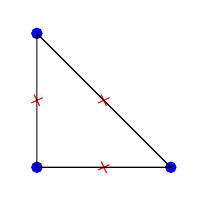
\begin{tikzpicture}[scale=1.7]

    \coordinate (0) at (0,0);
    \coordinate (1) at (1,0);
    \coordinate (2) at (0,1);

    \coordinate (3) at (0,0.5);
    \coordinate (4) at (0.5,0.5);
    \coordinate (5) at (0.5,0);

    \foreach \i in {0,1, 2}
    \draw[blue,fill=blue] (\i) circle (1.1pt) node [below] {};

    \foreach \i in {3,4,5}
    \draw (\i) node[cross, draw=red, rotate=-20] {};


    \draw (0) --(1) -- (2) -- (0);

  \end{tikzpicture}
  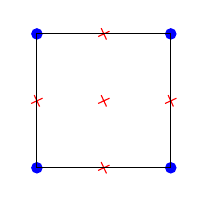
\begin{tikzpicture}[scale=1.7]

    \coordinate (0) at (0,0);
    \coordinate (1) at (1,0);
    \coordinate (2) at (1,1);
    \coordinate (3) at (0,1);


    \coordinate (4) at (0.5,0,0);
    \coordinate (5) at (1.0,0.5);
    \coordinate (6) at (0.0,0.5);
    \coordinate (7) at (0.5,1.0);
    \coordinate (8) at (0.5,0.5);

    \foreach \i in {0,1, 2, 3}
    \draw[blue,fill=blue] (\i) circle (1.1pt) node [below] {};


    \foreach \i in {4,5,6,7,8}
    \draw (\i) node[cross, draw=red, rotate=-20] {};


    \draw (0) --(1) -- (2) -- (3) -- (0);

  \end{tikzpicture}
  \qquad\qquad
  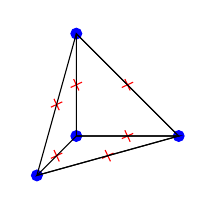
\begin{tikzpicture}[scale=1.3]

    \coordinate (0) at (0,0,0);
    \coordinate (1) at (1,0,0);
    \coordinate (2) at (0,1,0);
    \coordinate (3) at (0,0,1);

    \coordinate (4) at (0.5,0,0);
    \coordinate (5) at (0,0.5,0);
    \coordinate (6) at (0,0,0.5);
    \coordinate (7) at (0.5,0.5,0.0);
    \coordinate (8) at (0.5,0.0,0.5);
    \coordinate (9) at (0.0,0.5,0.5);


    \foreach \i in {0,1,2,3}
    \draw[blue,fill=blue] (\i) circle (1.5pt) node [below] {};


    \foreach \i in {4,5,6,7,8,9}
    \draw (\i) node[cross, draw=red, rotate=-20] {};


    \draw (0) -- (1) -- (2) -- (0);
    \draw (0) -- (1) -- (3) -- (0);
    \draw (1) -- (2) -- (3) -- (1);

  \end{tikzpicture}
  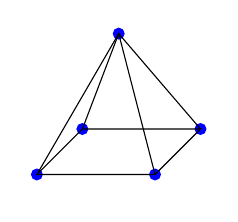
\begin{tikzpicture}[scale=1.5]

    \coordinate (0) at (0.0, 0.0, 0.0);
    \coordinate (1) at (0.0, 0.0, 1.0);
    \coordinate (2) at (1.0, 0.0, 0.0);
    \coordinate (3) at (1.0, 0.0, 1.0);
    \coordinate (4) at (0.5, 1.0, 0.5);

    \coordinate  (5) at (0.5, 0.0, 0.0);
    \coordinate  (6) at (0.0, 0.0, 0.5);
    \coordinate  (7) at (0.5, 0.0, 1.0);
    \coordinate  (8) at (1.0, 0.0, 0.5);

    \coordinate  (9) at (0.25,0.5,0.25);
    \coordinate (10) at (0.25,0.5,0.75);
    \coordinate (11) at (0.75,0.5,0.25);
    \coordinate (12) at (0.75,0.5,0.75);


    \coordinate (13) at (0.5, 0.0, 0.5);

    \foreach \i in {0,1,2,3,4}
    \draw[blue,fill=blue] (\i) circle (1.3pt) node [below] {};


    %\foreach \i in {5, 6, 7, 8, 9, 10, 11, 12, 13}
    %    \draw (\i) node[cross] {};


    \draw (0) -- (1) -- (3) -- (2) -- (0);
    \draw (1) -- (4) -- (3);
    \draw (0) -- (4) -- (2);

  \end{tikzpicture}
  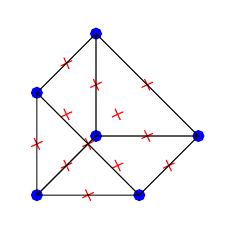
\begin{tikzpicture}[scale=1.3]

    \coordinate (0) at (0,0,1.5);
    \coordinate (1) at (1,0,1.5);
    \coordinate (2) at (0.0,1.0,1.5);

    \coordinate (3) at (0,0,0);
    \coordinate (4) at (1,0,0);
    \coordinate (5) at (0.0,1.0,0);



    \coordinate  (6) at (0.5, 0.0, 0.0);
    \coordinate  (7) at (0.0, 0.5, 0.0);
    \coordinate  (8) at (0.5, 0.5, 0.0);

    \coordinate   (9) at (0.5, 0.0, 0.75);
    \coordinate  (10) at (0.0, 0.5, 0.75);
    \coordinate  (11) at (0.5, 0.5, 0.75);

    \coordinate  (12) at (0.5, 0.0, 1.5);
    \coordinate  (13) at (0.0, 0.5, 1.5);
    \coordinate  (14) at (0.5, 0.5, 1.5);
  
    \coordinate (15) at (0,0,0.75);
    \coordinate (16) at (1,0,0.75);
    \coordinate (17) at (0.0,1.0,0.75);

    \foreach \i in {0,1,2,3,4,5}
    \draw[blue,fill=blue] (\i) circle (1.5pt) node [below] {};

    \foreach \i in {6,7,8,9,10,11,12,13,14,15,16,17}
    \draw (\i) node[cross, draw=red, rotate=-20] {};


    \draw (0) -- (1) -- (2) -- (0);
    \draw (3) -- (4) -- (5) -- (3);
    \draw (0) -- (3);
    \draw (1) -- (4);
    \draw (2) -- (5);

  \end{tikzpicture}
  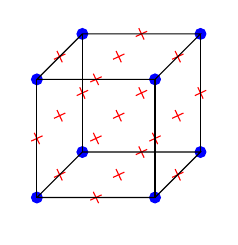
\begin{tikzpicture}[scale=1.5]

    \coordinate (0) at (0,0,1);
    \coordinate (1) at (1,0,1);
    \coordinate (2) at (0,0,0);
    \coordinate (3) at (1,0,0);

    \coordinate (4) at (0,1,1);
    \coordinate (5) at (1,1,1);
    \coordinate (6) at (0,1,0);
    \coordinate (7) at (1,1,0);

    \coordinate  (8) at (0,0,0.5);
    \coordinate  (9) at (1,0,0.5);
    \coordinate (10) at (0.5,0,1);
    \coordinate (11) at (0.5,0,0);
    \coordinate (12) at (0.5,0,0.5);

    \coordinate (13) at (0,1,0.5);
    \coordinate (14) at (1,1,0.5);
    \coordinate (15) at (0.5,1,1);
    \coordinate (16) at (0.5,1,0);
    \coordinate (17) at (0.5,1,0.5);


    \coordinate (18) at (0,0.5,1);
    \coordinate (19) at (1,0.5,1);
    \coordinate (20) at (0,0.5,0);
    \coordinate (21) at (1,0.5,0);
    \coordinate (22) at (0,0.5,0.5);
    \coordinate (23) at (1,0.5,0.5);
    \coordinate (24) at (0.5,0.5,1);
    \coordinate (25) at (0.5,0.5,0);
    \coordinate (26) at (0.5,0.5,0.5);



    \foreach \i in {0,1,2,3,4,5,6,7}
    \draw[blue,fill=blue] (\i) circle (1.3pt) node [below] {};

    \foreach \i in {8,9,10,11,12,13,14,15,16,17,18,19,20,21,22,23,24,25,26}
    \draw (\i) node[cross, draw=red, rotate=-20] {};


    \draw (0) -- (1) -- (3) -- (2) -- (0);
    \draw (4) -- (5) -- (7) -- (6) -- (4);
    \draw (0) -- (4);
    \draw (1) -- (5);
    \draw (2) -- (6);
    \draw (3) -- (7);

  \end{tikzpicture}

  \caption{\it Reference cells in 2D (triangle, quadrilateral) and 3D
    (tetrahedron, pyramid, wedge, hexahedron) with the support points
    indicated both for linear ({\color{blue}$\bullet$}) and quadratic
    ({\color{red}$\times$}) shape functions.
  %\todo[inline]{The pyramid is missing red crosses. The wedge is
  %  missing them on three edges.}
  % PM: we only have linear pyramids for now.
  }
  \label{fig:simplex}
\end{figure}

\begin{table}
  \caption{\it List of new scalar \texttt{FiniteElement} classes for the new
  reference-cell types. Vectorial elements can be constructed based on these classes
  via \texttt{FE\_Systems}.}\label{tab:simplex:fe}
  \centering
  \begin{tabular}{cccc}
    \toprule
    \textbf{reference cell} & \textbf{finite element} & \textbf{dimension} & \textbf{degree}\\
    \midrule
    \multirow{2}{*}{simplex (line, triangle, tetrahedron)} & FE\_SimplexP, FE\_SimplexDGP  & 1--3 & 1--2 \\
                                          & FE\_SimplexP\_Bubbles  & 1--3 & 1--2 \\
    pyramid & FE\_PyramidP, FE\_PyramidDGP  & 3 & 1 \\
    wedge & FE\_WedgeP, FE\_WedgeDGP  & 3 & 1--2 \\
    \bottomrule
  \end{tabular}
\end{table}


\subsubsection{Refactoring of internal data structures}

To enable simplex and mixed mesh support, we performed a major refactoring of the internal data structures of \dealii. In particular, the \texttt{Triangulation} class and
the \texttt{DoFHandler} class have undergone large changes and now
support meshes composed of all of the cells shown in Fig.~\ref{fig:simplex}.

The template parameters of the internal data structures of \texttt{Triangulation}
have been removed and the type of each cell and of each face (only in 3D) is stored. The function
\texttt{Triangulation::create\_\allowbreak triangulation()}, which converts a given list of
cells and vertices to the internal data structures, has been rewritten
inspired by \citep{logg2012} and this has had the side effect of a speed-up of up to 5. Minor adjustments
have also been made to the \texttt{parallel::shared::Triangulation}
and \texttt{parallel::\allowbreak fullydistributed::\allowbreak
  Triangulation} classes such that
the new mesh types can also be used in parallel.

The internal data structures of \texttt{DoFHandler} used to be hard-coded for pure
hypercube meshes, while the \texttt{hp::DoFHandler} used to be built around
CRS-like data structures. Due to the need of CRS data structures in the
\texttt{DoFHandler} in the context of more general meshes, we have merged
\texttt{hp::DoFHandler} into the \texttt{DoFHandler}. The class \texttt{hp::DoFHandler}, which is now a dummy derivation of \texttt{DoFHandler}, currently only exists for compatibility reasons and has
been deprecated, see Section~\ref{subsec:deprecated}. It will be
removed in the next release.

\subsubsection{Generating meshes}

The most obvious way to generate a simplex or a mixed mesh is to read the mesh from a file
generated by an external mesh generator. Currently, we support the
\texttt{VTK}, \texttt{MSH} (generated by the \textsc{gmsh} program \cite{geuzaine2009gmsh}), and \texttt{EXODUS II} file formats.

Alternatively, one can create a pure hypercube mesh with the existing functions
in the \texttt{GridGenerator} namespace and convert it to a
pure simplex mesh with the function
\texttt{GridGenerator::convert\_\allowbreak hypercube\_\allowbreak to\_\allowbreak simplex\_\allowbreak mesh()}.

\subsubsection{Using simplex meshes}

After having created a triangulation, one can proceed in the same way
as for hypercube meshes. In particular, one selects an appropriate finite element, mapping, and
quadrature class as follows:

\begin{c++}
FE_SimplexP<dim, spacedim> fe(degree);
MappingFE<dim, spacedim> mapping(FE_SimplexP<dim, spacedim>(1));
QGaussSimplex<dim> quad(degree + 1);

DoFHandler<dim> dof_handler(tria);
dof_handler.distribute_dofs(fe);

FEValues<dim, spacedim> fe_values(mapping, fe, quad, flags);
\end{c++}
The  list of currently supported finite-element classes is provided in Table~\ref{tab:simplex:fe}. Currently,
only linear and quadratic mappings via the \texttt{MappingFE} and
\texttt{MappingFEField} classes built around the listed nodal elements are available.
%\todo[inline]{I don't understand the previous sentence. "linear" means
%  p=1, but isoparametric means that it has the same p as the finite
%  element. It can't be both.}
For quadrature, the classes \texttt{QDuffy}, \texttt{QGaussSimplex}, \texttt{QWitherdenVincentSimplex} \cite{schloemer21, witherden2015identification},
\texttt{QGaussPyamid}, and \texttt{QGaussWedge} are
available.

\subsubsection{Using mixed meshes}
For mixed meshes, concepts known from the $hp$-context have been applied:
 different finite-element classes are assigned to different cells
 based on their respective kind of reference cell. In the
case of a 2D mixed mesh, which can only consist of triangles and
quadrilaterals, the finite element defined on a triangle (e.g., \texttt{FE\_SimplexP})
and on a quadrilateral (e.g., \texttt{FE\_Q}) can be collected in a \texttt{hp::FECollection}:

\begin{c++}
hp::FECollection<dim, spacedim> fe
  {FE_SimplexP<dim, spacedim>(degree), FE_Q<dim, spacedim>(degree)};
\end{c++}

Similarly, \texttt{hp::QCollection} and \texttt{hp::MappingCollection} can be used
to construct appropriate collections. Furthermore, the correct active
finite element index, which points to the correct
finite element of that cell, has to be assigned to each cell. The
following piece of code will then correctly enumerate all degrees of
freedom on the mesh:

\begin{c++}
DoFHandler<dim> dof_handler(tria);

for (const auto &cell : dof_handler.active_cell_iterators())
  switch (cell->reference_cell_type())
    {
      case ReferenceCell::Type::Tri:  cell->set_active_fe_index(0); break;
      case ReferenceCell::Type::Quad: cell->set_active_fe_index(1); break;
      // 3D (Tet, Pyramid, Wedge, Hex) not shown
      default: Assert(false, ExcNotImplemented());
    }

dof_handler.distribute_dofs(fe);
\end{c++}

\subsubsection{Practical implications}

The introduction of simplex and mixed meshes leads to some implications
for the user if these features are to be used. For instance, each cell might have a different type with
different number of vertices, lines, and faces so that these quantities can not be
compile-time constants anymore. This information used to be queried from
the \texttt{GeometryInfo} class. To avoid using this class, we have extended
relevant classes, e.g., \texttt{TriaAccessor} or \texttt{TriaCellAccessor},
with useful new functions like \texttt{n\_vertices()}, \texttt{n\_lines()}, or
\texttt{n\_faces()} so that users can simply write:
\begin{c++}
for (const auto &cell : tria.active_cell_iterators())
  for (unsigned int f = 0; f < cell->n_faces(); ++f)
    // do something with cell->face(f);
\end{c++}
Alternatively, one can use an iterator-based approach to loop over all faces
of a cell, introduced in the previous release. The relevant functions have been adjusted to be able to deal with
the now variable number of faces per cell:
\begin{c++}
for (const auto &cell : tria.active_cell_iterators())
  for (const auto &face : cell->face_iterators())
    // do something with face
\end{c++}
Furthermore, for mixed meshes, the number of degrees of freedom will differ between cells so that
cell-local arrays need to be resized for each
cell (as has previously already been the case in the $hp$-context):
\begin{c++}
std::vector<double> local_rhs;
for (const auto &cell : dof_handler.active_cell_iterators())
 {
   hp_fe_values.reinit(cell);
   local_rhs.resize(cell->get_fe().n_dofs_per_cell());
 }
\end{c++}


What is true for cells is also true for faces in 3D: faces can be either triangles
or quadrilaterals. This is the case even if no mixed mesh is used if
the mesh consists exclusively of pyramids or wedges. As a consequence, some functions, e.g. \texttt{FiniteElementData::n\_dofs\_per\_face()}, have been extended with a new optional argument for the face number.

Geometric information about cells and faces -- previously provided by
the \texttt{GeometryInfo} class for hypercube-type cells -- is now
available via the  \texttt{ReferenceCell} class that can be
instantiated for each of the seven possible reference cell. The
correct reference cell object for a cell or face can be obtained, respectively, using
\texttt{cell->reference\_cell()}, and either the call
\texttt{cell->reference\_cell().face\_reference\_cell(f)}
or
\texttt{cell->face(f)->reference\_cell()}.

Furthermore, many functions in \dealii{} used mappings that, when not
given explicitly, defaulted to (bi-/tri-)linear ones. These no longer
work for simplex or mixed meshes, and in these cases users will need
to explicitly provide the correct mapping for the mesh to be used.


\subsubsection{Matrix-free support}

\dealii{}'s matrix-free support has also been extended to simplex and
mixed meshes, for both
continuous and discontinuous elements. From a user perspective, the main
changes are to pass a $d$-dimensional quadrature object (rather than
one for 1D),
and the fact that \texttt{FEEvaluation} and \texttt{FEFaceEvaluation} must not
specify the polynomial degree via template arguments, determining all
information at runtime. More details can be found in
Section~\ref{subsec:mf}.

For the current release, no advanced algorithms for evaluating values and
gradients at quadrature points, such as sum factorization, are used.
The use of full interpolation matrices is for now acceptable since only low-order elements are
supported.



%%%%%%%%%%%%%%%%%%%%%%%%%%%%%%%%%%%%%%%%%%%%%%%%%%%%%%%%%%%%%%%%%%%%%%%%%%%%%%%%
\subsection{Advances in the particle infrastructure}
\label{subsec:particles}

\dealii 's particle infrastructure has been modernized to store nearly all
particle data as a collection of continuous data arrays instead of a container of
objects. This reorganization improves cache efficiency when iterating over
particles and reduces the amount of data that needs to be moved when a particle
moves to a different cell. Keeping track of unused data slots allows to reuse
them for new particles, significantly reducing memory allocations when
particles are created after other particles have left the local domain. The
data arrays are rebuilt and sorted during every mesh refinement cycle.

Additionally, the particle infrastructure now supports a faster search algorithm
for particles that moved farther than one cell width between particle sorting
operations, and support for updating ghost particles (particles that live in
ghost cells around the local domain) by updating their properties instead of
destroying and rebuilding their container. The latter step improves the
efficiency of ghost particle exchange significantly. With this feature,
\dealii can be used for scalable parallel Lagrangian
models such as the Discrete Element Method (DEM) \cite{golshan2021lethedem}
or Molecular Dynamics.

Finally, the \texttt{Particles::DataOut} class now supports writing particle
properties as vectors or tensors instead of a collection of scalars if the properties are
marked as such.


%%%%%%%%%%%%%%%%%%%%%%%%%%%%%%%%%%%%%%%%%%%%%%%%%%%%%%%%%%%%%%%%%%%%%%%%%%%%%%%%
\subsection{Advances in the multigrid infrastructure}
\label{subsec:mg}

Until now, \dealii has only supported ``local smoothing'' multigrid
algorithms~\citep{ClevengerHeisterKanschatKronbichler2019} wherein
smoothers only act on the cells of a given refinement level,
skipping those parts of the mesh that have not been adaptively refined
to that level. This approach guarantees that the work done summed up
over all levels is proportional to the number of unknowns, and is
consequently necessary so that the overall multigrid preconditioner
can have a complexity of ${\cal O}(N)$.

In contrast, the current release now also supports ``global
coarsening'' algorithms \citep{becker2000multigrid, sundar2012parallel} when
using continuous (\texttt{FE\_Q}, \texttt{FE\_SimplexP}) and
discontinuous (\texttt{FE\_DGQ}, \texttt{FE\_SimplexDGP})
elements. Global coarsening builds multigrid levels for the entire
domain, coarsening \textit{all} cells of a triangulation regardless of
how many times they have been refined. In addition, the framework now available in
\dealii{} is not only applicable to geometric coarsening, but can also
perform coarsening by reducing the polynomial degree ($p$-multigrid,
see~\cite{Fehn2020}), for example
to support $hp$-adaptive meshes.
%where it has been shown that one can
%efficiently precondition high-order spaces with lower-order finite
%element operators.
% MK: I do not think "precondition" is a precise enough description of p-multigrid
% because one still needs smoothing on the fine levels in addition to the
% "solve" at the coarser degree, a fact not transported by the mere
% 'precondition' term; rather than trying to discuss this in a more precise way,
% let us simply skip it as that is not central to the presentation here.
Finally, the implementation also supports transfer between continuous
and discontinuous elements as a further way to create multigrid levels.

These new multigrid variants promise fewer solver
iterations and better parallel scalability than the existing local
smoothing algorithms, but have to deal with
hanging nodes within each level and general require more computational
work per iteration overall.

The transfer operators between two levels have been implemented in the new class \texttt{MGTwoLevel\allowbreak Transfer}, which can be set up via the functions \texttt{MGTwoLevel\allowbreak Transfer::\allowbreak reinit\_\allowbreak geometric\_\allowbreak transfer()} or \texttt{MGTwo\allowbreak LevelTransfer::\allowbreak reinit\_\allowbreak polynomial\_\allowbreak transfer()} for given
\texttt{DoFHandler} and \texttt{AffineConstraints} objects
corresponding to the two levels. The resulting transfer operators
can then be collected in a single
\texttt{MGTransfer\allowbreak GlobalCoarsening} object that can be used just as the previous workhorse \texttt{MGTransferMatrixFree} within the \texttt{Multigrid}
algorithm.
%Several common operations are encoded in utility
%functions in the \texttt{MGTransferGlobalCoarseningTools}
%namespace.
To facilitate the construction of matrix diagonals with matrix-free methods as well as a matrix representation of the coarse level matrix, new utility functions \texttt{create\_diagonal()} and \texttt{create\_matrix()} from
the \texttt{MatrixFreeTools} namespace have been added (see also Subsection~\ref{subsec:mf}).

The usage of the new transfer operators (and of some of the utility
functions) in the context of a hybrid multigrid algorithm
($hp$-multigrid with algebraic multigrid as coarse-grid solver) for $hp$-problems is demonstrated in the new tutorial \texttt{step-75}, see also Section~\ref{subsec:steps}.



%%%%%%%%%%%%%%%%%%%%%%%%%%%%%%%%%%%%%%%%%%%%%%%%%%%%%%%%%%%%%%%%%%%%%%%%%%%%%%%%
\subsection{Advances in the matrix-free infrastructure}
\label{subsec:mf}

\dealii{}'s matrix-free framework enables high-throughput operations
for applications in which only the availability of the \textit{action}
of a matrix, but not the entries of the matrix, are necessary. This
framework has been substantially extended in the current release.


\subsubsection{Precompilation of evaluation kernels}

The \texttt{FEEvaluation} and \texttt{FEFaceEvaluation} classes use template parameters for
the polynomial degree of the finite element $k$ and the number of the 1D quadrature points $q$
to generate near-optimal code for these operations.
For application codes that rely on operators of many different degrees (e.g., because
they use $p$-multigrid or $hp$-algorithms), creating all instantiations
can be overly complex and incur long compile times.

In the current release, specializations of these classes that do
not rely on the template parameters $k$ and $q$ (expressed in the code
using special values ``-1'' and ``0'') have been added. For example:
\begin{c++}
FEEvaluation<dim, -1, 0, n_components, Number, VectorizedArrayType>
  phi(range, dofhandler_index, quadrature_index, first_selected_component);
\end{c++}
These classes select at runtime -- for common low and medium
polynomial degree/quadrature combinations ($k\le 6$ and $q\in\{ k+1,
k+2, \left\lfloor (3k)/2 \right\rfloor \}$) -- efficient precompiled implementations and default to non-templated
evaluation kernels otherwise (see also \texttt{FEEvaluation::fast\_evaluation\_\allowbreak supported()}).

In the case that even higher polynomial degrees are needed, one can precompile the
relevant internal classes
(\texttt{FEEvaluationFactory}, \texttt{FEFaceEvaluationFactory}, \texttt{CellwiseInverseMassFactory}) in the user code for needed \texttt{degree}s
and \texttt{VectorizedArrayType}s in the following way:
\begin{c++}
#define FE_EVAL_FACTORY_DEGREE_MAX 12

#include <deal.II/matrix_free/evaluation_template_factory.templates.h>

DEAL_II_NAMESPACE_OPEN
template struct dealii::internal::FEEvaluationFactory
  <dim, VectorizedArrayType::value_type, VectorizedArrayType>;
// same for FEFaceEvaluationFactory and CellwiseInverseMassFactory (skipped)
DEAL_II_NAMESPACE_CLOSE
\end{c++}


\subsubsection{Parallel matrix-free $hp$-implementation}\label{subsubsection:mf:hp}

With release 9.1, large parts of the $hp$-algorithms
in \dealii were ported to a model that allows for
parallel matrix-based simulations \cite{dealII91}. In the present
release, the parallel $hp$ support was extended to \texttt{MatrixFree}.

Until now, the \texttt{FEEvaluation} classes used the template
parameters $k$ and $q$ to select the correct active FE and quadrature
index and users were responsible for the cumbersome detection of 
subranges of the same $k$ and $q$ within the cell ranges returned by the 
matrix-free loops.
%\todo{I don't understand what ``detection of subranges of the same
%  degree'' refers to. Please clarify. In particular, I don't know what
%``subranges'' mean in this paragraph.}
The creation of subranges is now performed internally, and the non-templated versions
of the \texttt{FEEvaluation} classes have been extended for the $hp$-case. To determine
the desired FE and quadrature index of a subrange, the current cell/face range has to be provided
to the constructors of the \texttt{FEEvaluation} classes. These changes enable
users to write matrix-free code independently of whether $hp$-capabilities are used or not.

The new tutorial \texttt{step-75} presents how to use the new $hp$-related features in \texttt{MatrixFree}
in the context of a hybrid-multigrid solver.



\subsection{MPI-3.0 shared-memory support}\label{subsec:sm}
In many large computations, certain pieces of data are computed
(or read from disk) once and then treated as read-only. If this information is needed by more
than one MPI process, it is more efficient to store this information only
once in shared memory among all processes located on a multicore
node. MPI supports the creation of such shared memory windows since
version 3.0, and deal.II can now use this in the
\texttt{AlignedVector} and \texttt{Table} classes that are often used
for large lookup tables for classes such as \texttt{InterpolatedTensorProductGridData}.

Shared memory storage is also used in the \texttt{MatrixFree} and
\texttt{LinearAlgebra::\allowbreak distributed::\allowbreak Vector} classes. If \texttt{MatrixFree} has been configured by setting
\texttt{MatrixFree::\allowbreak AdditionalData::\allowbreak communicator\_sm} appropriately, then
\texttt{MatrixFree::create\_dof\_vector()} creates vectors that share
information among all processes on one node. As a consequence, the
\texttt{FEEvaluation} classes can access vector elements owned by
other processes and in certain cases node-local
communication can be skipped. To prevent race conditions, \texttt{MatrixFree} uses local
barriers at the beginning and the end of loops (\texttt{loop()}, \texttt{cell\_loop()}, \texttt{loop\_cell\_centric()}).

The new \texttt{step-76} tutorial program illustrates this case
in the context of the solution of the Euler equations. It reaches a
speed-up of 27\% compared to the
original version, \texttt{step-67}, by using the new feature.
For more details and the usage of the feature in the library \texttt{hyper.deal}, see \citep{munch2020hyperdeal}.



%%%%%%%%%%%%%%%%%%%%%%%%%%%%%%%%%%%%%%%%%%%%%%%%%%%%%%%%%%%%%%%%%%%%%%%%%%%%%%%%
\subsection{Evaluation and integration at arbitrary points}
\label{subsec:fepointvalues}

In a number of circumstances, finite element solutions need to be evaluated at
arbitrary reference points that change from one element to next. Two important
examples are particle simulations coupled to a finite element solution, or
algorithms on non-matching grids. The existing \texttt{FEValues} class is a poor
fit for this task, as it is based on the assumption that evaluation of
shape functions and their derivatives happens at the same quadrature
points on every cell, and that consequently expensive computations can
be done once and results re-used for many subsequent cells. The new class
\texttt{FEPointEvaluation} provides a more convenient interface for
cases where the evaluation on different cells does not happen at the
same points mapped from the reference cell.
For tensor product finite elements (\texttt{FE\_Q}, \texttt{FE\_DGQ})
and tensor product mappings (\texttt{MappingQGeneric} and derived classes),
the new approach is also very fast, as it can use some of the matrix-free
infrastructure and vectorization facilities.

As an example, let us consider the evaluation of a
surface tension force in the context of sharp-interface methods, whose
contribution is added to a fluid solver by multiplication with test function
and addition over quadrature points located at the interface section
$\Gamma_K=\Gamma \cup K$ of the current cell $K$ and that is,
in general, positioned differently within $K$ than for any other cell:
\begin{align*}
\left(\mathbf{v}, \kappa \, \mathbf{n}\right)_\Gamma
\approx
\sum_q \mathbf{v}(\mathbf{x}_q) \cdot \left(\kappa(\mathbf{x}_q) \, \mathbf{n}(\mathbf{x}_q)\right) (JxW)_q.
\end{align*}
In \dealii{}, this can now be conveniently written as
\begin{c++}
phi_curvature.reinit(cell, reference_points);
phi_normal.reinit(cell, reference_points);
phi_force.reinit(cell, reference_points);

phi_curvature.evaluate(curvature_values, EvaluationFlags::values);
phi_normal.evaluate(normal_values, EvaluationFlags::values);

for (unsigned int q = 0; q < n_points; ++q)
  phi_force.submit_value(phi_curvature.get_value(q) *
                         phi_normal.get_value(q) * JxW[q], q);
                          
phi_force.integrate(force_values, EvaluationFlags::values);
\end{c++}
The quadrature points (at reference positions
\texttt{reference\_points}) and the related \texttt{JxW} value can,
for example, come from
a mesh of lower dimension. Determining to which \texttt{cell} a quadrature
point belongs to on the background mesh, including the reference cell
coordinates \texttt{reference\_\allowbreak points}, is aided by functions like
\texttt{find\_active\_cell\_around\_point()}
\texttt{find\_all\_active\_cells\_\allowbreak around\_\allowbreak point()} from the \texttt{GridTools} namespace. While these
functions have been available in \dealii{} previously, their performance has
been considerably enhanced with the aforementioned more optimized code paths
for selected mappings.

While \texttt{FEPointEvaluation} assumes that evaluation points are already sorted according to 
the owning cells and thus can focus on cell-local operations, the new class
\texttt{RemotePointEvaluation} is responsible for determining the owning cells in a distributed
context and for providing efficient communication patterns for the data exchange. In \texttt{deal.II},
the class has been successfully applied together with \texttt{FEPointEvaluation} to evaluate a distributed
solution vector at arbitrary points (see also the
\texttt{VectorTools::point\_values()} function).


%%%%%%%%%%%%%%%%%%%%%%%%%%%%%%%%%%%%%%%%%%%%%%%%%%%%%%%%%%%%%%%%%%%%%%%%%%%%%%%%
\subsection{Simplified implementation for face integrals}
\label{subsec:feinterfacevalues}
Discontinuous Galerkin (DG) methods -- and other methods with penalty
terms defined on faces -- require the evaluation of averages and jumps
across cell faces, involving values and derivatives of the shape
functions and solutions from two adjacent cells. The
\texttt{FEInterfaceValues} class, first introduced in \dealii{} 9.2,
is designed to provide the necessary interface.

Internally, this class provides an abstraction for two
\texttt{FEFaceValues} objects (or \texttt{FESubfaceValues} when using
adaptive refinement). The class introduces new interface degrees of
freedom indices that are the union of the degrees of freedom indices
of the two \texttt{FEFaceValues} objects. The interface degrees of
freedom indices can be converted to the corresponding local degrees of
freedom indices of the two cells using a helper function. New in the
current release is better support for vector-valued problems: scalar
or vector components of shape functions can now be extracted by providing an \texttt{FEValuesExtractors} object.


%%%%%%%%%%%%%%%%%%%%%%%%%%%%%%%%%%%%%%%%%%%%%%%%%%%%%%%%%%%%%%%%%%%%%%%%%%%%%%%%
\subsection{The source-based toolchain installer \candi{}}
\label{subsec:candi}

The requirement to download, compile, and install \dealii{} and its dependencies from
source is a major obstacle to many \dealii{} users.
Compiling all dependencies from source can be difficult but is a necessity on operating systems for which
binary packages aren't available or on compute clusters and other machines
without root privileges for the user to install system dependencies.

The source based installation of \dealii{} and its many dependent libraries
can be done with the \candi{} script tool for various
Linux operating systems, within the Windows Subsystem Linux (WSL), and
on OS X (experimental).
%
The general assumption is that a C, C++ and Fortran compiler and suitable MPI-compilers
for the base compilers as well as the corresponding development system packages are
available.

\candi is a bash-script based tool, is an abbreviation of ``compile and install''
and is released under the GNU LGPL v3.0.
%
The origin of \candi{} is a fork made in 2013 from \texttt{dorsal},
a now-retired source based installer for the \texttt{FEniCS} library.
%
The \candi{} tool can be found via the download page of \dealii{} since version 8.5
or from \url{github.com/dealii/candi}, and is under active development.
To install older releases of \dealii{} toolchains, one can check out
the \candi{} branch of the \texttt{git} repository that
corresponds to the desired \dealii{} version.

\candi{} downloads, unpacks, compiles, and installs an individual
library (called a ``package'' in \candi{}), a list of libraries, or a complete toolchain.
The toolchain installation is the default behavior and the default configuration
ensures that most of the \dealii{} step tutorials can be used directly.
The package installation mode is also useful to generate docker containers.
In toolchain mode, \candi{} checks for and deals with
dependencies between libraries appropriately.

Each package for a library is defined by variables for its name and version,
a (remote or local) download location,
its packaging format (e.g. tar, gz, or zip),
a checksum,
its general build chain (e.g., using \texttt{autotools}, \texttt{cmake}, or others),
as well as configuration options.
Moreover, one can give specific instructions for each of the steps being
necessary for the unpacking, configuration, or building of a package.
A new feature allows \candi{} to skip user prompts, allowing its use in
a batch mode.

\candi{} does all this by either downloading packages from the
internet, including through mirrors, or re-using previously downloaded
or checked out from a repository.
If temporary files of \candi{} are not removed, one can use the developer
mode to prepare patches or developments for any of the packages.

\candi{} is organized in the following way:
\begin{itemize}
\item \texttt{candi.sh}: the bash script which controls the overall process.
Available command line options are listed by calling ``\texttt{candi.sh -h}''
and explained in the \texttt{README.md} file.

\item \texttt{candi.cfg} (or \texttt{local.cfg}): the default toolchain
configuration file. Here one can easily switch on/off features,
give additional configuration, and
list the packages for a toolchain.

\item \texttt{deal.II-toolchain} folder: the central project folder for
\dealii{}-based toolchains.
It contains subfolders
for packages (libraries, dependencies, general tools in a specific version),
platforms (operating systems) and
for patches to be applied after unpacking a package.
\end{itemize}

The installer is developed in the \texttt{dealii/candi}
\texttt{github} repository, and uses continuous
integration (CI) to ensure that old and new features
are working as expected.


%%%%%%%%%%%%%%%%%%%%%%%%%%%%%%%%%%%%%%%%%%%%%%%%%%%%%%%%%%%%%%%%%%%%%%%%%%%%%%%%
\subsection{New and improved tutorials and code gallery programs}
\label{subsec:steps}

Many of the \dealii{} tutorial programs were revised in a variety of
ways as part of this release. In addition, there are a number of new tutorial programs:
\begin{itemize}
\item \texttt{step-19} is an introductory demonstration of \dealii{}'s
  particle functionality. It solves the coupled problem of
  charged particles and an electric field, using a cathode tube as an
  example.

\item \texttt{step-66} shows how to solve a nonlinear problem using Newton's method in the matrix-free
framework in parallel. The PDE considered is the Gelfand problem $-\triangle u = \exp(u)$.
  
\item \texttt{step-68} is a demonstration of how to embed and distribute
  particles in a parallel triangulation. It tracks the movement of
  a set of particles in a fluid flow and illustrates how to distribute
  a parallel domain according to the number of locally owned
  particles instead of the number of locally owned cells.

\item \texttt{step-71} focuses on automatic and symbolic
  differentiation (AD and SD, in short) as a tool to make solvers for complex,
  nonlinear problems possible. To this end, \dealii{} can interface to a number
  of AD and SD libraries, specifically Trilinos' Sacado package
  \cite{Bartlett2006a}, ADOL-C \cite{Griewank1996a}, and
  SymEngine \cite{symengine-web-page}. The tutorial
  illustrates how these techniques can be used to compute derivatives
  first of a rather simple function, and then of the much more complex
  energy functions of two magnetoelastic and magneto-viscoelastic
  material formulations in which just the scalar energy functional
  takes up the better part of a page, and even first derivatives can
  only be computed with heroic effort.

\item \texttt{step-72} illustrates the use of automatic
  differentiation to simplify the computation of derivatives in the
  context of nonlinear partial differential equations where one needs
  to compute the Jacobian from the residual operator for efficient
  Newton iterations. \texttt{step-72} builds on the minimal surface
  solver \texttt{step-15} and replaces the hand-construction of the
  Jacobian by either computing it as the derivative of the residual,
  or alternatively as the second derivative of an energy functional
  that then also yields the residual itself.

\item \texttt{step-74} implements the symmetric interior penalty Galerkin 
(SIPG) method for Poisson's equation using the \texttt{FEInterfaceValues} class
within the \texttt{MeshWorker::mesh\_loop()} framework. This tutorial demonstrates a
simple to assemble face integrals.

  
\item \texttt{step-75} demonstrates a state-of-the-art way of solving a simple
      Laplace problem using $hp$-adaptation and hybrid multigrid methods on machines
      with distributed memory. This tutorial points out particularities in porting
      serial $hp$-adaptive code for parallelization. Furthermore, it guides through
      the process of writing an efficient preconditioner for $hp$-adaptive applications.

\item \texttt{step-76} is an explicit time integrator for the
      compressible Euler equations discretized with a high-order discontinuous
      Galerkin (DG) scheme, using the matrix-free infrastructure just as \texttt{step-67} does.
      The tutorial presents advanced topics, like the usage of cell-centric loops and
      the new MPI-3.0 shared-memory capabilities of \texttt{MatrixFree} to reach high
      throughput. Furthermore, the utilization of the template parameter
      \texttt{VectorizedArrayType} and the application of lambda functions to describe cell and face
      integrals are discussed.

\item \texttt{step-77} is a program that illustrate \dealii{}'s
  interfaces to the SUNDIALS library \cite{sundials}, and specifically
  the KINSOL nonlinear solver. Like the \texttt{step-72} program
  mentioned above, it is a variation of the minimal surface solver
  \texttt{step-15}: Instead of implementing the nonlinear Newton and
  line search loop ourselves, \texttt{step-77} relies on KINSOL for
  decisions such as when to rebuild the Jacobian matrix, when to
  actually solve linear systems with it, and how to form updates that
  drive the residual to convergence. The program illustrates the
  substantial savings that can be obtained by not re-inventing the
  wheel but instead building on an existing and well-tuned software
  such as KINSOL.

  \dealii{}'s interfaces to the various SUNDIALS sub-packages were also updated to the latest SUNDIALS release, 5.7.

\item \texttt{step-78}, a program written by Tyler Anderson at
  Colorado State University, solves the
  one-dimensional Black-Scholes equations to model the price of stock
  options.

\item \texttt{step-79} is a program for topology optimization. Written
  by Justin O'Connor at Colorado State University, the program asks
  what the optimal distribution of a finite amount of material in a
  domain is to maximize its strength (or optimize some other objective
  functional). It uses advanced optimization techniques to deal with
  the nonlinearity of the problem as well as with the equality and
  inequality constraints that characterize the application.
\end{itemize}

There is also a new program in the code gallery (a collection of
user-contributed programs that often solve more complicated problems
than tutorial programs, and intended as starting points for further
research rather than as teaching tools):
\begin{itemize}
\item ``\texttt{Laplace equation coupled to an external simulation program}'' was
  contributed by David Schneider and Benjamin Uekermann at Technical University
  of Munich. It extends \texttt{step-4} to a time-dependent Poisson
  problem and couples it with a simple external surface-based
  application, using the \texttt{preCICE} 
  library~\cite{bungartz2016precice, lindner2020exafsa}. \texttt{preCICE},
  also allows to couple \dealii to external simulation packages, 
  such as OpenFOAM, SU2, CalculiX, or FEniCS, using adapter classes. 
  The webpage
  \url{https://precice.org/} provides several more \dealii{}-based tutorials,
  including interesting fluid-structure interaction applications.
\end{itemize}



%%%%%%%%%%%%%%%%%%%%%%%%%%%%%%%%%%%%%%%%%%%%%%%%%%%%%%%%%%%%%%%%%%%%%%%%%%%%%%%%
\subsection{Incompatible changes}\label{subsec:deprecated}

The 9.3 release includes
\href{https://dealii.org/developer/doxygen/deal.II/changes_between_9_2_0_and_9_3_0.html}
{around 45 incompatible changes}; see \cite{changes93}. The majority of these changes
should not be visible to typical user codes; some remove previously
deprecated classes and functions; and the majority change internal
interfaces that are not usually used in external
applications. That said, the following are worth mentioning since they
may have been more widely used:
\begin{itemize}
  \item The \texttt{hp::DoFHandler} class has been deprecated. The standard
        \texttt{DoFHandler} class is now capable of all $hp$-functionalities.
  \item Consequently, all template arguments \texttt{DoFHandlerType} are obsolete,
        and classes like \texttt{DataOut} or \texttt{SolutionTransfer} for example
        no longer require them. If you rely on these template arguments, an interim
        namespace \texttt{Legacy} has been introduced that provides all affected
        classes with the old interface for a transition period.
\end{itemize}



%%%%%%%%%%%%%%%%%%%%%%%%%%%%%%%%%%%%%%%%%%%%%%%%%%%%%%%%%%%%%%%%%%%%%%%%%%%%%%%%
%%%%%%%%%%%%%%%%%%%%%%%%%%%%%%%%%%%%%%%%%%%%%%%%%%%%%%%%%%%%%%%%%%%%%%%%%%%%%%%%
%%%%%%%%%%%%%%%%%%%%%%%%%%%%%%%%%%%%%%%%%%%%%%%%%%%%%%%%%%%%%%%%%%%%%%%%%%%%%%%%
\section{How to cite \dealii}\label{sec:cite}

In order to justify the work the developers of \dealii{} put into this
software, we ask that papers using the library reference one of the
\dealii{} papers. This helps us justify the effort we put into this library.

There are various ways to reference \dealii{}. To acknowledge the use of
the current version of the library, \textbf{please reference the present
  document}. For up to date information and a bibtex entry
see
\begin{center}
  \url{https://www.dealii.org/publications.html}
\end{center}

The original \dealii{} paper containing an overview of its
architecture is \cite{BangerthHartmannKanschat2007}, and a more recent
publication documenting \dealii{}'s design decisions is available as \cite{dealII2020design}. If you rely on
specific features of the library, please consider citing any of the
following:
\begin{multicols}{2}
  \vspace*{-36pt}
  \begin{itemize}
    \item For geometric multigrid: \cite{Kanschat2004,JanssenKanschat2011,ClevengerHeisterKanschatKronbichler2019};
    \item For distributed parallel computing: \cite{BangerthBursteddeHeisterKronbichler11};
    \item For $hp$-adaptivity: \cite{BangerthKayserHerold2007};
    \item For partition-of-unity (PUM) and finite element enrichment methods:
           \cite{Davydov2016};
    \item For matrix-free and fast assembly techniques:
          \cite{KronbichlerKormann2012,KronbichlerKormann2019};
    \item For computations on lower-dimensional manifolds:
          \cite{DeSimoneHeltaiManigrasso2009};
    \item For curved geometry representations and manifolds:
          \cite{HeltaiBangerthKronbichlerMola2019};
    \item For integration with CAD files and tools:
          \cite{HeltaiMola2015};
    \item For boundary element computations:
          \cite{GiulianiMolaHeltai-2018-a};
    \item For the \texttt{LinearOperator} and
      \texttt{Packaged\-Operation} facilities:
          \cite{MaierBardelloniHeltai-2016-a,MaierBardelloniHeltai-2016-b};
    \item For uses of the \texttt{WorkStream} interface:
          \cite{TKB16};
    \item For uses of the \texttt{ParameterAcceptor} concept, the
          \texttt{MeshWorker::ScratchData} base class, and the
          \texttt{ParsedConvergenceTable} class:
          \cite{SartoriGiulianiBardelloni-2018-a};
    \item For uses of the particle functionality in \dealii{}:
          \cite{GLHPB18}.
          \vfill\null
  \end{itemize}
\end{multicols}

\dealii{} can interface with many other libraries:
\begin{multicols}{3}
  \begin{itemize}
    \item ADOL-C \cite{Griewank1996a,adol-c}
    \item ArborX \cite{lebrun2020arborx}
    \item ARPACK \cite{arpack}
    \item Assimp \cite{assimp}
    \item BLAS and LAPACK \cite{lapack}
    \item cuSOLVER \cite{cusolver}
    \item cuSPARSE \cite{cusparse}
    \item Gmsh \cite{geuzaine2009gmsh}
    \item GSL \cite{gsl2016}
    \item Ginkgo \cite{ginkgo-web-page}
    \item HDF5 \cite{hdf5}
    \item METIS \cite{karypis1998fast}
    \item MUMPS \cite{ADE00,MUMPS:1,MUMPS:2,mumps-web-page}
    \item muparser \cite{muparser-web-page}
    \item OpenCASCADE \cite{opencascade-web-page}
    \item p4est \cite{p4est}
    \item PETSc \cite{petsc-user-ref,petsc-web-page}
    \item ROL \cite{ridzal2014rapid}
    \item ScaLAPACK \cite{slug}
    \item SLEPc \cite{Hernandez:2005:SSF}
    \item SUNDIALS \cite{sundials}
    \item SymEngine \cite{symengine-web-page}
    \item TBB \cite{Rei07}
    \item Trilinos \cite{trilinos,trilinos-web-page}
    \item UMFPACK \cite{umfpack}
  \end{itemize}
\end{multicols}
Please consider citing the appropriate references if you use
interfaces to these libraries. 

The two previous releases of \dealii{} can be cited as
\cite{dealII91,dealII92}.


\section{Acknowledgments}

\dealii{} is a world-wide project with dozens of contributors around the
globe. Other than the authors of this paper, the following people
contributed code to this release:\\
%
% Uwe Koecher doesn't usually show up in the changelog, but
% we should make sure he's listed.
%
% 9.3: updated 5/08/2021 PM
%      sorted by WB 5/28
Pasquale Africa,
Tyler Anderson,
Mathias Anselmann,
Arpit Babbar,
Maximilian Bergbauer,
Nicolas Barnafi,
Michele Bucelli,
Marcus Calhoun-Lopez,
Fabian Castelli, %He provided major contributions to candi for v9.3
Praveen Chandrashekar,
Conrad Clevenger,
David F. Castellanos,
Andrew Davis,
Elias Dejene,
Niklas Fehn,
Menno Fraters,
Ivan Fumagalli,
Daniel Garcia-Sanchez,
Nicola Giuliani,
Krishnakumar Gopalakrishnan,
Alexander Grayver,
Olivier Guevremont,
Jake Harmon,
Graham Harper,
Katharina Kormann,
Christoph Kammer,
Wenyu Lei,
Zhou Lei,
Phillip Mobley,
Nils Much,
Pratik Nayak,
Toni El Geitani Nehme,
Justin O'Connor,
Daniel Paukner,
Lei Qiao,
Ce Qin,
Reza Rastak,
Julian Roth,
Laura Prieto Saavedra,
Doug Shi-Dong,
David Schneider,
Magdalena Schreter,
Richard Schussnig,
Dominic Soldner,
Simon Sticko,
Malhar Tidke,
Ignacio Tomas,
Peter Westerbaan.

Their contributions are much appreciated!


\bigskip

\dealii{} and its developers are financially supported through a
variety of funding sources:

D.~Arndt and B.~Turcksin: Research sponsored by the Laboratory Directed Research and
Development Program of Oak Ridge National Laboratory, managed by UT-Battelle,
LLC, for the U. S. Department of Energy.

W.~Bangerth, T.~Heister, R.~Gassm{\"o}ller, and J.~Zhang were partially
supported by the Computational Infrastructure for Geodynamics initiative
(CIG), through the National Science Foundation (NSF) under Award
No.~EAR-1550901 and The University of California -- Davis.

W.~Bangerth and M.~Fehling were partially supported by Award OAC-1835673
as part of the Cyberinfrastructure for Sustained Scientific Innovation (CSSI)
program.

W.~Bangerth was also partially supported by Awards DMS-1821210 and EAR-1925595.

B.~Blais was partially supported by the National Science and Engineering
Research Council of Canada (NSERC)  through the RGPIN-2020-04510 Discovery
Grant

T.~Heister and J.~Zhang were also partially supported by NSF
Award OAC-2015848.

T.~Heister was also partially supported by the NSF Awards DMS-2028346,
EAR-1925575, and by Technical Data Analysis, Inc. through US Navy STTR
Contract N68335-18-C-0011.

R.~Gassm{\"o}ller was also partially supported by the NSF Award
EAR-1925595.

L.~Heltai was partially supported by the Italian Ministry of Instruction,
University and Research (MIUR), under the 2017 PRIN project NA-FROM-PDEs MIUR
PE1, ``Numerical Analysis for Full and Reduced Order Methods for the efficient
and accurate solution of complex systems governed by Partial Differential
Equations''.

M.~Kronbichler and P.~Munch were partially supported by the
Bayerisches Kompetenznetzwerk
f\"ur Technisch-Wissen\-schaft\-li\-ches Hoch- und H\"ochstleistungsrechnen
(KONWIHR) in the context of the projects
``Performance tuning of high-order discontinuous Galerkin solvers for
SuperMUC-NG'' and ``High-order matrix-free finite element implementations with
hybrid parallelization and improved data locality''.

M.~Maier was partially supported by NSF Awards DMS-1912847 and DMS-2045636.

D.~Wells was supported by NSF through Grant DMS-1344962.

The Interdisciplinary Center for Scientific Computing (IWR) at Heidelberg
University has provided hosting services for the \dealii{} web page.

\bibliography{paper}{}
\bibliographystyle{abbrv}

\end{document}
